
\section{Finanzplanung}
Hier erläutern wir die Hauptkostenarten sowie Einnahmequellen und entsprechende Annahmen, mit deren Hilfe wir zu einer realistischen Einschätzung der Cashflows der ersten zwei Jahre gelangen.
\subsection{Umsatz}
Als Umsatz werden für die Schätzung lediglich die Einnahmen aus den Abonnements betrachtet. Zusätzlich sollten an dieser Stelle auch Werbeeinnahmen addiert werden, die wir jedoch mangels genauer Prognosen weglassen. Es handelt sich hier also um eine konservative Schätzung.\\
Neben den kalkulierten Preisen für private Accounts (1\euro{} basic, 3\euro{} extended) und Firmenkunden (150\euro{} basic, 450\euro{} extended) nehmen wir außerdem je Kundengruppe einen Split von 30-70 für den Kauf der extended- bzw. der basic-Version an. Der Marktanteil wird konservativ mit 1\% angesetzt, was einer realistischen Schätzung für ein Spezial-Start-Up in den ersten 24 Monaten entspricht.
\subsection{Hauptkostenarten}
Im ersten Monat fallen Lizenzkosten in Höhe von 35.000\euro{} an. Dazu kommen relativ geringfügige Fixkosten der GmbH-Anmeldung. In den darauf folgenden 4 Monaten spielen die Kosten des externen Development-Dienstleisters eine wichtige Rolle. \\
Den bei weitem größten laufenden Posten bilden die Personalkosten, gefolgt von den variablen Kosten der IT-Infrastruktur bei Amazon Web Services. 

\subsection{Szenario-Analyse}
Ausgehend von dem Normalfall werden das beste und schlechteste Szenario durch Variation der Umsatzerlöse simuliert. Die Kosten nehmen wir dabei jeweils als konstant an. Von der Besteuerung wird an dieser Stelle abgesehen und stattdessen nur der EBIT betrachtet. Im Überblick zeigt Abbildung \ref{fig:financials1} den Verlauf der Kosten, Umsatzerlöse und des Gewinns vor Steuern und Abschreibungen (EBIT) im neutralen Umsatzszenario. \\
Für jedes Szenario ist die Lage des Break-Even-Punktes von besonderem Interesse (Tabelle \ref{tab:break-even}):
\\
\\
\begin{table}[h!]
  \centering
    \begin{footnotesize}
  \begin{tabular}{|l|l|l|l|}\hline
  \textbf{ } &  \textbf{Umsatz (relativ)} &  \textbf{Break-Even} \\ \hline
 \textbf{best case} & 150\% & 12. Monat \\ \hline
\textbf{neutral case} & 100\% & 18. Monat \\ \hline
 \textbf{worst case} & 50\% & 25. Monat \\ \hline
  \end{tabular} 
    \end{footnotesize}
  \caption{Break-Even in Szenarien mit unterschiedlicher Umsatzentwicklung}
  \label{tab:break-even}
\end{table} 
\\
\\
\\
\begin{figure}[h!]
\centering
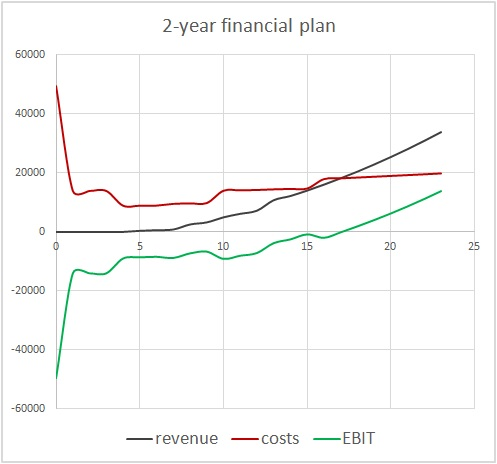
\includegraphics[width=0.7\textwidth]{financials}
\caption{Umsatz, Kosten und EBIT im neutralen Fall der Umsatzentwicklung}
\label{fig:financials1}
\end{figure}

\subsection{Detaillierte Finanzplanung}
Im Folgeden werden die Details des Finanzplans anhand des neutralen Szenarios näher betrachtet. Hier wird der Break-Event-Punkt in Monat 18 erreicht. In der Betrachtung der Kosten werden auch die Umsatzgebühren des Microtransaction-Dienstleisters PayPal berücksichtigt. In Abbildung \ref{fig:financials2} werden die einzelnen Kostenarten sowie Umsatzquellen und zusätzliche Parameter aufgeführt, die ein neutrales Umsatzszenario beschreiben. 
\begin{figure}[h!]
\centering
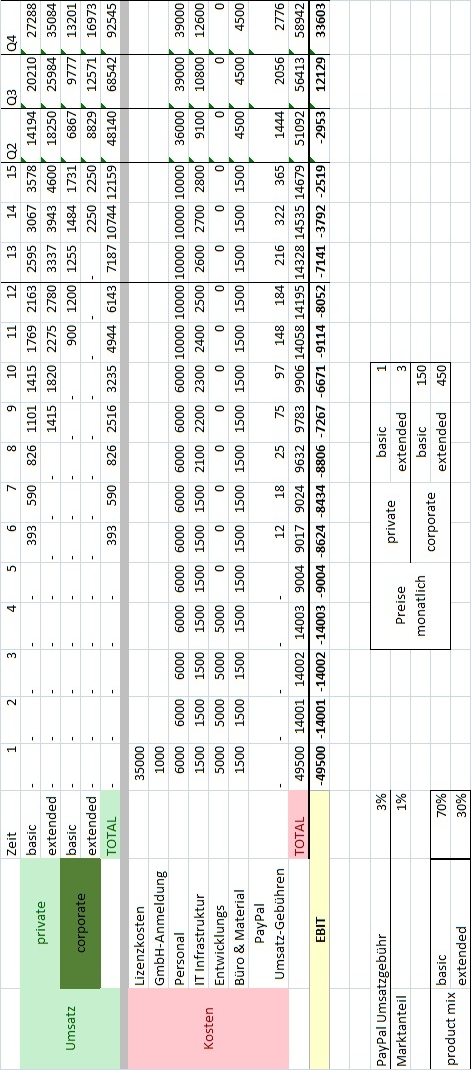
\includegraphics[width=0.6\textwidth]{finance-table}
\caption{Detaillierter Finanzplan für das neutrale Umsatz-Szenario.}
\label{fig:financials2}
\end{figure}
\\
\\
\\
\\
\\
\\
\\
\\
\\
\section{Schlusswort}
Das Gründerteam von SemLit ist zuversichtlich, dass Sie von unserem Erfolg überzeugt sind. Wir blicken entschlossen in die Zukunft und freuen uns auf eine erfolgreiche Zusammenarbeit. 
\\
\\
\\
\\
\\
\\
\\
\\
Igor Tseyzer und Artem Schumilin
